 %!TeX root = ../main.tex
\chapter{总结与展望}
\section{工作总结}
本文主要研究内容是对逃逸电子动理学过程进行数值分析,完成了动理学数值计算平台以及电子回旋辐射数值诊断平台。同时,通过结合动理学和对应的电子回旋辐射演化,本文模拟了两种放电条件下电子回旋辐射现象,并分析了其背后的物理机制。另一方面,本论文还通过保体积算法详细分析了电子与电磁波相互作用过程中的反常多普勒效应,发现了电磁波对逃逸电子的约束能量阈值,并提出了用于抑制逃逸电子能量的方法。


\noindent	\textbf{本文具体研究内容总结如下:} 
\begin{enumerate}
\item
分析了反常多普勒效应(ADE)产生的物理机制,发现了ADE的阈值电场并提出了新的抑制逃逸电子的方法。电子回旋辐射信号的台阶结构目前主流观点认为是ADE,当电子速度与电磁波满足$ω=\vk∙\vv+ω_{ce}$时即发生ADE。为了理解这个过程,本文利用VPA算法模拟了电子与电磁波相互作用过程,发现导致ADE效应主要由左旋电磁波构成。当左旋电磁波电场强度超过背景加速电场约3倍时,外界电磁波可将电子平行方向静电场能量散射到垂直方向,同时电子还会激发出和背景电磁波相同性质的电磁波,电子平行方向速度此时始终保持共振条件不再受静电场加速。这一发现为托卡马克中利用电磁波抑制逃逸电子提供了思路。通过对冷等离子体本征模分析,本文发现处于上杂化频率附近的电磁波最容易满足共振要求,该区间本征波原则上可以有效抑制逃逸电子能量,并且相关实验论文也发现在电子速度出现迅速散射时观测到上杂化频率电磁波\cite{RN786,RN1868}。基于以上发现,本文提出通过托卡马克装置高场侧注入电磁波激发上杂化频率有可能对逃逸电磁形成平行磁场方向的速度屏障,抑制逃逸电子能量。
\item
开发了针对非热电子动理学理论的数值计算平台和以及电子回旋辐射计算平台,程序框图如\autoref{fig:programframe}所示。本文动理学所采用的方法是将电子分为主体电子和试探电子,其中主体电子处于热平衡态,试探电子通过动理学模型求解。目前已经有许多研究人员提出动理学模型来描述过不同物理过程,从Landreman的简化版Fokker-Plank碰撞项到Pike的精确的碰撞项,从A.Stahl的粒子守恒版的回旋辐射阻尼项到O.Embreus的大角度Boltzmann碰撞项,本文的理论模型主要基于以上研究成果,分别考虑电场项、电子小角度碰撞项、电子雪崩碰撞项以及电子回旋辐射阻尼项等过程。利用面向对象编程,通过谱方法和半隐式算法求解动理学方程,实现了非热化电子演化的动理学数值模拟,通过标准模型校验,如双温演化、洛伦兹气体扩散等模型验证了数值解的可靠性,通过和Kulsrud基于低温下Fokker-Plank方程中初级逃逸电子增长率的数值计算\cite{RN2095}结果对比验证了理论模型的一致性和算法的精确性;关于电子回旋辐射的数值计算,本文主要建立在B A Trubnikov\cite{RN1414}	和G. Bekefi\cite{RN1337}等理论基础,并且验证了由B A Trubnikov理论得到的光学厚度数值结果和Bornatici的理论结果\cite{RN351}	的一致性,最后定性分析了光学厚度对电子回旋辐射的影响。
\begin{figure}[ht]
\centering
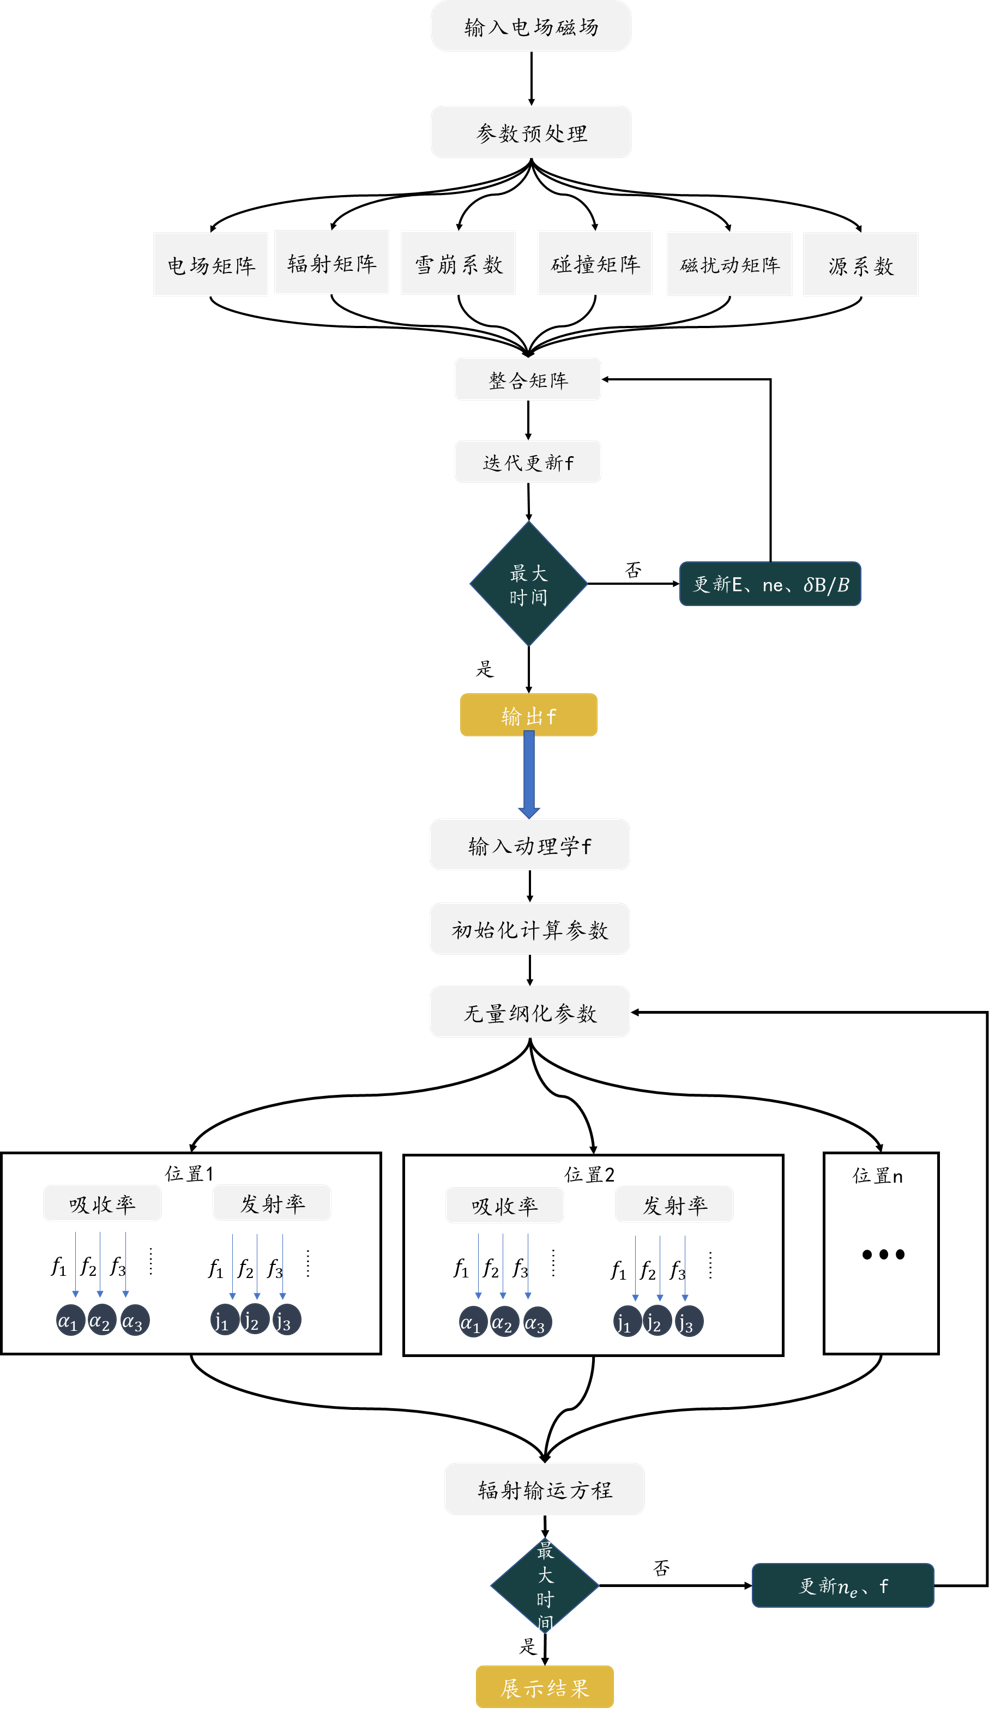
\includegraphics[width=14cm]{codeframe.png}
\caption{\label{fig:programframe}动理学与电子回旋辐射数值诊断联合仿真计算平台}
\end{figure}

\item
利用数值平台解释了放电初级电子回旋辐射前端峰的形成以及密度下降过程中回旋辐射突然指数增长的物理机制。通过非热化电子动理学演化的数值平台和电子回旋辐射数值模型,本文对放电过程中电子回旋辐射前端峰形成过程进行了模拟,发现在前端峰产生过程中逃逸电子雪崩效应起到了不可或缺的作用;关于密度下降过程中电子回旋辐射突然指数上升现象,本文通过模拟和实验研究发现随机磁扰动是导致该过程电子回旋辐射变化的主要原因。随机磁扰动会破坏等离子体中逃逸电子的约束,当密度下降时,磁扰动突然降低,导致逃逸电子约束变好,非热化电子辐射才迅速上升,实验数据和模拟也证明了这一点。
\end{enumerate}
\noindent	\textbf{本文创新点总结如下:} 
\par 本论文动理学求解方法结合了CODE的谱方法和NORSE程序的面向对象编程思想实现了空间维度为0D2P(零个位置空间,两个动量空间)分布函数演化数值计算,其中包含了电场驱动项,试探粒子碰撞项、回旋辐射阻尼项、以及目前最完备的逃逸电子雪崩项等物理过程,可以根据放电过程中密度、环电压等时变背景参数研究动理学方程的动态演化过程。相对于过去的动理学计算程序,本论文的计算方法兼顾了计算效率,结合时下最完备的雪崩算符,利用面向对象编程技术可用于求解动态背景环境中非热化电子分布函数的演化过程。本论文首次展示了ECE信号前端峰的形成与逃逸电子雪崩效应的关联。关于放电平台期通过对密度调控使其下降达到某一阈值时电子回旋辐射突然上升的现象,之前的研究解释为雪崩效应的双阈值现象,本论文提出了完全不同观点,认为该现象与磁扰动有关,并通过数值模拟和实验数据验证了这个观点。
\par 通过对电子和电磁波相互作用的模拟并结合色散关系分析,本论文发现了可实现约束逃逸电子的电磁波能量阈值,并提出了利用非寻常波约束逃逸电子的方法。非寻常波在等离子体中朗道阻尼小,更容易通过反常多普勒效应抑制逃逸电子,而低杂波朗道阻尼较大,更适合用于加热背景电子,不同的波模对应不同能量的电子。通过较高能量的低杂波加热背景电子和较低能量非寻常波抑制逃逸电子,理论上实现了加热效率和逃逸电子能量约束双赢,该方法对提高托卡马克放电品质、保护装置等方面均有值得期待的探索价值。

\section{前景展望}
在未来的托卡马克放电过程中,随着放电参数的不断提高,逃逸电子的影响也会越来越显著,因此对逃逸电子的动理学过程的理解也更加重要。本文中的动理学模型主要有以下问题仍可继续优化:
\begin{enumerate}
\item
该模型只能采用具有温度分布的等离子体背景环境下动理学分析,没有考虑主体电子的动理学演化过程,这导致文中动理学程序无法计算等离子体加热过程。该模型适用于电场强度远小于$E_D$电场的等离子体环境,这种电场不会影响等离子体主体电子速度分布,因此该模型同样无法模拟托卡马克放电破裂过程中动理学行为。在未来我们将进一步考虑主体等离子体的动理学机制,使之能应用于更宏观的等离子体物理过程研究,如加热、破裂等过程。
\item
由于电磁湍动算符复杂度高,难度大,目前还没有实现对动理学方程中ADE的数值求解,对辐射step结构的解释并没有完成。革命尚未成功,作为本论文的第一推动力,在未来的时间将继续探究这个问题,这不仅是因为这种具有类似量子化特征的台阶结构本身很奇特,更重要的是逃逸电子激发的电磁波和逃逸电子自身的相互作用的物理过程对控制逃逸电子保护装置有重要的研究价值。
\item

动理学模型可以进一步考虑逃逸电子与环电压的耦合,环电压的变化和逃逸电子实际上是互相影响的,环电压因逃逸电子增加而下降,逃逸电子因环电压下降而减小,二者之间构成了负反馈系统。因此如果我们能够把环电压和动理学耦合在一起,同时考虑主体等离子体动理学演化,这样就可以研究等离子体放电过程中逃逸电子自洽的演化过程,这个过程在等离子体形成和破裂过程中起到了举足轻重的作用。

\end{enumerate}





























